%-------------------------------------------------------------------------------
% Autores: I. R. Pagnossin e Centro de Ensino e Pesquisa Aplicada.
%
% Este material é parte integrante do curso "Usando LaTeX; pensando em TeX" e é
% distribuido pelos autores segundo a licença Creative Commons 2.5 Brasil
% (atribuição/não-comercial/redistribuição segundo a mesma licença).
%
% This material is part of the course "Usando LaTeX; pensando em TeX".
% It is distributed according to the license Creative Commons 2.5 Brazil
% (attribution/non-comercial use/share alike the same license).
%-------------------------------------------------------------------------------
\newif\ifhandout
%\handouttrue  % Descomente se for para gerar a versão para IMPRESSÃO.
\handoutfalse % Descomente se for para gerar a versão para APRESENTAÇÃO

%-------------------------------------------------------------------------------
\ifhandout
  \documentclass[handout,10pt]{beamer}
  \mode<handout>
\else
	\documentclass[10pt,hyperref={pdfpagelabels=false}]{beamer}
	\mode<presentation>
\fi

	\usepackage[utf8]{inputenc}
	\usepackage[brazil]{babel}	
	\usepackage{graphicx}
	\usepackage{listings}
	\usepackage{tikz}
	\usepackage{amsmath}
	\usepackage[squaren]{SIunits}	
	\usepackage{fancybox}
	\usepackage{array}
	\usepackage{colortbl}		
	\usepackage{bookman}
	\usepackage{fancybox}
	\usepackage{booktabs}
	\usepackage{helvet}
	\usepackage{lipsum}
	\usepackage{tabularx}
	\usepackage{calc}
			
	\ifhandout
		\usepackage{pgfpages}
		\pgfpagesuselayout{2 on 1}[a4paper,border shrink=5mm]
	\fi

	% Bibliotecas TikZ e PGF necessárias
	\usetikzlibrary{shapes.symbols}
	\usepgflibrary{shapes.misc}
	\usetikzlibrary{calc}
	
	% Configurações pessoais
	% Configurações personalizadas do código LaTeX.	
\lstnewenvironment{LaTeXcode}{
	\setlength{\abovecaptionskip}{0pt}	
	\lstset{language=[LaTeX]TeX}
	\lstset{%
		basicstyle=\footnotesize\ttfamily,  % Global
		keywordstyle=\color{blue}\bfseries, % Comandos
		identifierstyle=,                   % Texto
		stringstyle=,                       % Strings 
		commentstyle=\color{gray},          % Comentários
		showstringspaces=false,             % Espaços
		rulecolor=\color{gray},             % Linha da caixa
	}
	\lstset{emph={setlength,includegraphics,psfrag,subfigure},emphstyle={\color{blue}\bfseries}}
}% Abrindo o ambiente.
{}% Fechando o ambiente.
	
\newcommand{\digite}[1]{{\fontfamily{cmss}\fontseries{bx}\selectfont#1}}	
\newcommand{\cs}[1]{{\normalfont\textbackslash\color{blue!50!black}#1}}
\newcommand{\pkg}[1]{{\normalfont\sffamily\color{orange}#1}}
\newcommand{\env}[1]{{\normalfont\sffamily\color{green!50!black}#1}}
\let\comando=\cs
\let\package=\pkg
\let\ambiente=\env
\newcommand{\foreign}[1]{{\textsl{#1}}}


	\newcounter{exercicio}	
	\newenvironment{exercicio}{%
		\refstepcounter{exercicio}%
		\penalty-200
		\noindent\colorbox{blue!60!black}{\makebox[\columnwidth-\fboxsep*2][c]{\textbf{\color{white}Exercício~\theexercicio}}}\smallskip
	}{\par\medskip}
		

\newcommand{\bibtex}{\textsc{Bib}\TeX}

\newenvironment<>{atividade}[1]{%
\begin{actionenv}#2%
\begin{exampleblock}{{Atividade #1}}%
}
{%
\end{exampleblock}%
\end{actionenv}%
}


	% Path das figuras, relativo a esta pasta.
	\graphicspath{{../arquivos_comuns/figuras/}{./figuras/}}

	% Modelo da apresentação	
	\usetheme{Frankfurt}
	\usefonttheme{serif,structurebold}
	%\setbeamercovered{transparent}		
		
	% Metadados do arquivo PDF.
	\hypersetup{
		pdftitle={Caixas},
		pdfauthor={Dr. Ivan R. Pagnossin},
		pdfsubject={LaTeX},
		pdfkeywords={TeX,LaTeX}
	}

	% Título, autores e instituição.
	\title{Caixas}
	\author{\textbf{Prof.:} Ivan R. Pagnossin \and \textbf{Tutora:} Juliana Giordano}
	\institute{%
		Coordenadoria de Tecnologia da Informação\\
		Centro de Ensino e Pesquisa Aplicada}
	\logo{
\includegraphics[width=0.25\textwidth]{LogotipoCursoLaTeX_v3_pequeno}}
	\date{}
	
	\newcommand{\scalefactor}{7}
	\tikzset{box/.style={color=#1,thick},box/.default=red}
	\tikzset{letter/.style={color=#1,inner sep=0pt},letter/.default=gray!50}
	\tikzset{baseline/.style={color=#1,thin},baseline/.default=blue}
		
	\newsavebox{\meuparbox}
	
\begin{document}
%-------------------------------------------------------------------
\begin{frame}[c,label=titulo]
	\centering	
	
	
\includegraphics[width=0.8\textwidth]{LogotipoCursoLaTeX_v2}

	\titlepage
\end{frame}
%-------------------------------------------------------------------
\logo{} % <-- O logotipo não aparecerá mais a partir daqui.
\setbeamertemplate{background canvas}{%
		
\includegraphics[width=\paperwidth,height=\paperheight,keepaspectratio=false]{leao-pensador-wattermark.png}
}
%-------------------------------------------------------------------
\section{Caixas}
\subsection{Dimensões}
\begin{frame}
	\frametitle{Definição e dimensões}

	\centering
	
	\begin{tikzpicture}

	% A letra "g" e sua caixa
	\node [letter] (g) at (2,0) {\scalebox{\scalefactor}
		{\color{gray!30}g}};
	\draw [box] (g.south west) rectangle (g.north east);
	
	\coordinate (base line left)  at ($(g.base west) - (5mm,0)$);
	\coordinate (base line right) at ($(g.base east) + (5mm,0)$);
	
	% A linha-base
	\draw [baseline] (base line left) -- (base line right);
			
	% A flecha e o rótulo "Linha-base"
	\draw [<-] ($(base line right) + (1mm,0)$) -- ++(5mm,0)
		node [inner sep=0mm, label=right:Linha-base] {};
	
	% O ponto-de-referência
	\fill [black] (g.base west) circle (3pt);
	
	% Flecha da altura
	\draw [<->] ($ (g.base west) + (-3mm,+0.5mm) $) --
	            ($ (g.north west) + (-3mm,0) $);
	
	% Flecha da profundidade
	\draw [<->] ($ (g.south west) + (-3mm,0) $) -- 
	            ($ (g.base west) + (-3mm,-0.5mm) $);

	% Flecha da largura
	\draw [<->] ($ (g.north west) + (0,3mm) $) --
	            ($ (g.north east) + (0,3mm) $);
	            
	% Flecha da altura total
	\draw [<->] ($ (g.south east) + (3mm,0) $) --
	            ($ (g.north east) + (3mm,0) $);
	
	% Rótulo "Altura"
	\node [inner sep=3mm, label=left:Altura]
		at ($ (g.base west)  ! 0.5 ! (g.north west) $) {};
	
	% Rótulo "Profundidade"
	\node [inner sep=3mm, label=left:Profundidade]
		at ($ (g.base west)  ! 0.5 ! (g.south west) $) {};
	
	% Rótulo "Largura"
	\node [inner sep=3mm, label=above:Largura]
		at ($ (g.north west) ! 0.5 ! (g.north east) $) {};
	
	% Rótulo "Altura total"
	\node [inner sep=3mm, label=right:Altura total]
		at ($ (g.base east)  ! 0.5 ! (g.north east) $) {};
	
	% Flecha e rótulo "Ponto-de-referência"
	\draw [<-] ($(g.base west) + (3pt,-3pt)$) -- ++(3mm,-3mm) -- ++(0mm,-1cm)
		node [circle,inner sep=0mm,label=below:Ponto-de-referência] {};
	
\end{tikzpicture}
		
	\vfill
				
	\uncover<2>{%----------------------------------------------------------------------------
	\begin{tikzpicture}[scale=\scalefactor]
		\node [letter] (A) {\scalebox{\scalefactor}{A}};
		\draw [box] (A.south west) rectangle (A.north east);
		
		\draw [baseline]
			($(A.base west) - (0.005\textwidth,0)$) --
			($(A.base east) + (0.005\textwidth,0)$);
		\fill (A.base west) circle (0.001\textwidth);
	\end{tikzpicture}\hfill					
%----------------------------------------------------------------------------
	\begin{tikzpicture}[scale=\scalefactor]
		\node [letter] (A) {\scalebox{\scalefactor}{%
			\makebox[0.2\width][l]{A}%
		}};
		\draw [box] (A.south west) rectangle (A.north east);
		
		\draw [baseline]
			($(A.base west) - (0.005\textwidth,0)$) --
			($(A.base east) + (0.005\textwidth,0)$);
		\fill (A.base west) circle (0.001\textwidth);
	\end{tikzpicture}\hfill
%----------------------------------------------------------------------------
	\begin{tikzpicture}[scale=\scalefactor]
		\node [letter] (A) {\scalebox{\scalefactor}{%
			\raisebox{0pt}[0pt][\height]{A}%
		}};
		\draw [box] (A.south west) rectangle (A.north east);
		
		\draw [baseline]
			($(A.base west) - (0.005\textwidth,0)$) --
			($(A.base east) + (0.005\textwidth,0)$);
		\fill (A.base west) circle (0.001\textwidth);
	\end{tikzpicture}			
%----------------------------------------------------------------------------}
	\ifhandout\else%
	\llap{\uncover<3>{\large\makebox[\textwidth]{
		\begin{columns}
			\centering
			\column{0.7\textwidth}
			\begin{block}{}
				Caixas são\dots
				\begin{itemize}
					\item flexíveis durante a construção
					\item rígidas após a construção
				\end{itemize}
			\end{block}
		\end{columns}}}}
	\fi
								
\end{frame}
%-------------------------------------------------------------------
\newsavebox{\demoboxes}
\begin{frame}[c]
	\frametitle{Exemplos de caixas no \LaTeX}
	\framesubtitle{Letras e linhas}
	
	\begin{center}
		
		%--------------------------------------------------------------
% Exercício 11.5 do livro TeXbook. A macro \demobox{<texto>} 
% substitui <texto> belos boxes construídos pelo TeX. Muito útil
% para compreender o conceito de box.
\def\dolist{\afterassignment\dodolist\let\next= }
\def\dodolist{\ifx\next\endlist \let\next\relax
  \else \\\let\next\dolist \fi
  \next}
\def\endlist{\endlist}
\def\hidehrule#1#2{\kern-#1%
  \hrule height#1 depth#2 \kern-#2 }
\def\hidevrule#1#2{\kern-#1{\dimen0=#1
  \advance\dimen0 by#2\vrule width\dimen0}\kern-#2 }
\def\makeblankbox#1#2{\hbox{\lower\dp0\vbox{\hidehrule{#1}{#2}%
  \kern-#1 % overlap the rules at the corners
  \hbox to \wd0{\hidevrule{#1}{#2}%
    \raise\ht0\vbox to #1{}% set the vrule height
    \lower\dp0\vtop to #1{}% set the vrule depth
    \hfil\hidevrule{#2}{#1}}%
  \kern-#1\hidehrule{#2}{#1}}}}
\def\maketypebox{\makeblankbox{0pt}{0.05pt}}
\def\makelightbox{\makeblankbox{.2pt}{.2pt}}
\def\\{\expandafter\if\space\next\
  \else \setbox0=\hbox{\next}\maketypebox\fi}
\def\demobox#1{\setbox0=\hbox{\dolist#1\endlist}%
  \copy0\kern-\wd0\makelightbox}
%--------------------------------------------------------------		
		\savebox{\demoboxes}{\large\demobox{%
		É assim que o \TeX\ enxerga o que	escrevemos:}}
		
		{\large É assim que o \TeX\ enxerga o que escrevemos:}\\
		\usebox{\demoboxes}
		
		\vspace{3em}
		
		\uncover<2->{%\documentclass{article}
%
%	\usepackage[utf8]{inputenc}
%	\usepackage{tikz}	
%	\usepackage{fourier}	
%	
%	\usetikzlibrary{calc}
%	
%\begin{document}
	%------------------------------------------------------------------
	% \raisebox{elevação}{g}
	%------------------------------------------------------------------
	\renewcommand{\scalefactor}{13}
	\colorlet{bcolor}{red!30}
	
	\begin{tikzpicture}[scale=\scalefactor]
				
		\coordinate (L) at (0,0);
		\coordinate (A) at (0.15em,0);
		\coordinate (T) at (0.54em,0);
		\coordinate (E) at (0.98em,0);
		\coordinate (X) at (1.47em,0);
	
		\node [inner sep=0pt,black!30] (nodeL) at (L)
			{\scalebox{\scalefactor}{L}};
			
		\node [inner sep=0pt,black!30] (nodeA) at (A)
			{\scalebox{\scalefactor}{\raisebox{+0.45ex}{\scriptsize A}}};
			
		\node [inner sep=0pt,black!30] (nodeT) at (T)
			{\scalebox{\scalefactor}{T}};
			
		\node [inner sep=0pt,black!30] (nodeE) at (E)
			{\scalebox{\scalefactor}{\raisebox{-0.47ex}[\height][\depth]{E}}};
			
		\node [inner sep=0pt,black!30] (nodeX) at (X)
			{\scalebox{\scalefactor}{X}};
		
		\draw [blue] ($ (nodeL.base west) - (0.3ex,0) $) --
		($ (nodeX.base east) + (0.3ex,0) $);
				
		\draw [red!100] (nodeL.south west) rectangle (nodeL.north east);
		\draw [blue!100] ($(nodeA.south west) + (0,0.02ex)$) rectangle
								($(nodeA.north east) - (0,0.02ex)$);
		\draw [red!100] (nodeT.south west) rectangle (nodeT.north east);
		\draw [blue!100] ($(nodeE.south west) - (0,0.45ex)$) rectangle
								($(nodeE.north east) - (0,0.45ex)$);
		\draw [red!100] (nodeX.south west) rectangle (nodeX.north east);
		
		\fill (nodeL.base west) circle (0.05ex);
		\fill ($(nodeA.south west) + (0,0.02ex)$) circle (0.05ex);
		\fill (nodeT.base west) circle (0.05ex);
		\fill (nodeE.base west) circle (0.05ex);
		\fill (nodeX.base west) circle (0.05ex);
		
		
	\end{tikzpicture}
	
%\end{document}}
	\end{center}
\end{frame}
%-------------------------------------------------------------------
\renewcommand{\scalefactor}{3}
\begin{frame}[c]
	\frametitle{Exemplos de caixas no \LaTeX}
	\framesubtitle{Parágrafos, páginas, figuras e tabelas}
	
	\begin{center}
	
		\begin{columns}
			\centering
		
			\column[t]{0.35\textwidth}
				\centering
			
					\begin{tikzpicture}

		% A letra "g" e sua caixa
		\node (g) %at (2,0)
			{\raisebox{-1cm}{%
				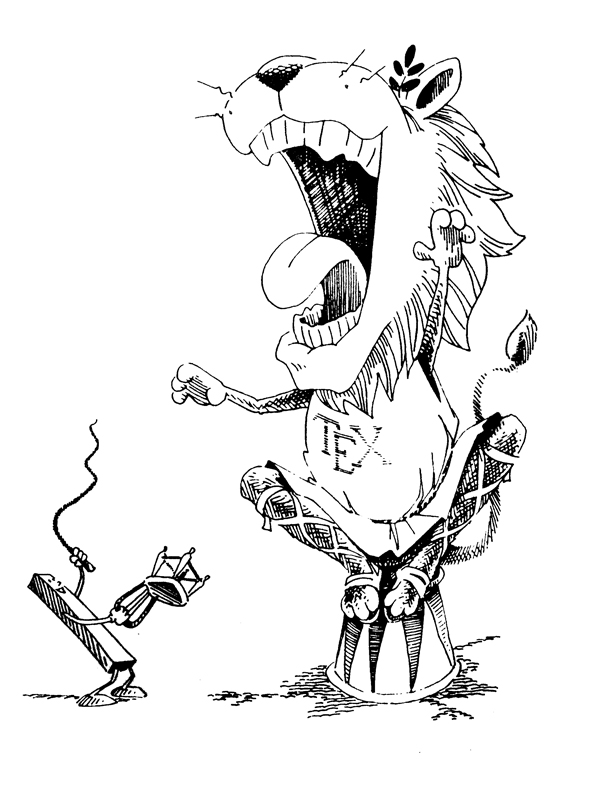
\includegraphics[width=\textwidth]{controlling_TeX_800x600}%
			}};
		%\draw [very thick,red!80] (g.south west) rectangle (g.north east);
		\draw [box] (g.south west) rectangle (g.north east);
		
		%\coordinate (base line left)  at ($(g.base west) - (5mm,0)$);
		%\coordinate (base line right) at ($(g.base east) + (5mm,0)$);
		
		% A linha-base
		%\draw [thick,blue] (base line left) -- (base line right);
		\draw [baseline] ($(g.base west) - (0.1\textwidth,0)$) --
										 ($(g.base east) + (0.1\textwidth,0)$);
				
		% A flecha e o rótulo "Linha-base"
		%\draw [<-,gray!50] ($(base line right) + (1mm,0)$) -- ++(5mm,0)
		%	node [inner sep=0mm, label=right:\textcolor{gray!50}{Linha-base}] {};
		
		% O ponto-de-referência
		\fill [black] (g.base west) circle (3pt);
		
		% Flecha da altura
		%\draw [<->,gray!50] ($ (g.base west) + (-3mm,+0.5mm) $) --
		%            ($ (g.north west) + (-3mm,0) $);
		
		% Flecha da profundidade
		%\draw [<->,gray!50] ($ (g.south west) + (-3mm,0) $) -- 
		%            ($ (g.base west) + (-3mm,-0.5mm) $);

		% Flecha da largura
		%\draw [<->,gray!50] ($ (g.north west) + (0,3mm) $) --
		%            ($ (g.north east) + (0,3mm) $);
		           
		% Flecha da altura total
		%\draw [<->,gray!50] ($ (g.south east) + (3mm,0) $) --
		%            ($ (g.north east) + (3mm,0) $);
		
		% Rótulo "Altura"
		%\node [inner sep=3mm, label=left:\textcolor{gray!50}{Altura}]
	  %		at ($ (g.base west)  ! 0.5 ! (g.north west) $) {};
		
		% Rótulo "Profundidade"
		%\node [inner sep=3mm, label=left:\textcolor{gray!50}{Prof.}]
		%	at ($ (g.base west)  ! 0.5 ! (g.south west) $) {};
		
		% Rótulo "Largura"
		%\node [inner sep=3mm, label=above:\textcolor{gray!50}{Largura}]
		%	at ($ (g.north west) ! 0.5 ! (g.north east) $) {};
		
		% Rótulo "Altura total"
		%\node [inner sep=3mm, label=right:\textcolor{gray!50}{Altura total}]
		%	at ($ (g.base east)  ! 0.5 ! (g.north east) $) {};
		
		% Flecha e rótulo "Ponto-de-referência"
		%\draw [<-,gray!50] ($(g.base west) + (3pt,-3pt)$) -- ++(3mm,-3mm) --
		 %++(0mm,-1cm)
			%node [circle,inner sep=0mm,label=below:\textcolor{gray!50}{Ponto-de-%
			%referência}] {};		
	\end{tikzpicture}
			
			\column[t]{0.55\textwidth}
				\centering
			
				\uncover<2->{%----------------------------------------------------------------------------
\savebox{\meuparbox}{\tiny\color{black!40}%
	\begin{tabular}{c|c|c}
		Camadas	&	Espessuras (\nano\metre) & Observações \\	\hline \hline
		GaAs & \multicolumn{2}{c}{Substrato semi-isolante (001)} \\ \hline
		GaAs & 50 & \foreign{Buffer} \\
		\hline
		$[(\text{AlAs})_5(\text{GaAs})_{10}]\times10$	&	84	&	Super-rede (SR)	\\
		\hline
		GaAs & 20 & \foreign{Buffer} \\
		\hline
		\color{blue!40} GaAs:Si & $\sim\unit{1}{mc}$ & 	
			$n_\text{Si}=\unit{4}{\times\terad\centi\rpsquare\metre}$ \\
		\hline
		\color{blue!40} GaAs & 30 & Barreira anterior \\
		\hline
		$\color{blue!40}\mathrm{In_yGa_{1-y}As}$ & 10 & QW
		 ($\mathrm{y}=16,534\%$)\\
		\hline
		\color{blue!40} GaAs & 7 & Barreira posterior \\
		\hline
		\color{blue!40} GaAs & 170 & \foreign{Buffer} \\
		\hline
		GaAs:Si & 10 & $\unit{3,0\times10^{17}}{\centi\rpcubic\metre}$ \\
		\hline
	\end{tabular}}		
%----------------------------------------------------------------------------
\begin{tikzpicture}
	\node (L) {\scalebox{0.85}{\usebox{\meuparbox}}};
	\draw [box] (L.south west) rectangle (L.north east);							

	% A linha-base
	\draw [baseline] ($(L.base west) - (0.05\textwidth,0)$) --
		($(L.base east) + (0.05\textwidth,0)$);

	% Ponto-de-referência
	\fill (L.base west) circle (0.015\textwidth);
	
\end{tikzpicture}}
				
				\uncover<3->{%----------------------------------------------------------------------------
\savebox{\meuparbox}{
	\begin{minipage}[t]{1.9\textwidth}
		\setlength{\parindent}{0.1\textwidth}
		\tiny\lipsum[1-3]
	\end{minipage}}
%----------------------------------------------------------------------------
\begin{tikzpicture}
	\node (L) {\scalebox{0.5}{\usebox{\meuparbox}}};
	\draw [box] (L.south west) rectangle (L.north east);	
	
	% A linha-base
	\draw [baseline] ($(L.base west) - (0.05\textwidth,0)$) --
				($(L.base east) + (0.05\textwidth,0)$);
				
	% Ponto-de-referência
	\fill (L.base west) circle (0.015\textwidth);
			
\end{tikzpicture}}
		\end{columns}
	\end{center}
	
\end{frame}
%-------------------------------------------------------------------
{
\renewcommand{\cs}[1]{{\ttfamily\textbackslash\textcolor{blue!50}{#1}}}
\renewcommand{\ambiente}[1]{{\ttfamily\textcolor{green!50}{#1}}}

\subsection{Tipos}
\begin{frame}[fragile]
	\frametitle{Caixas personalizáveis do \LaTeX}
		
	\begin{enumerate}
	
		\item<2-> \textbf{Caixas LR}
			(\foreign{left-right boxes})\\[-0.25\baselineskip]			
			{\scriptsize\color{gray!50}Os comandos \cs{fbox}, \cs{framebox},
			\cs{mbox}, \cs{makebox} e \cs{raisebox}.}
		
			\medskip
		
			\begin{center}\scriptsize
				\parbox{0.7\textwidth}{Você pode utilizar uma \fbox{caixa LR} no meio
				do texto. Ela pode ou não ter moldura, mas o importante é que ela
				\emph{não pode ser dividida}!}
			\end{center}
		
			\vfill
		
		\item<3-> \textbf{Caixas de parágrafo}
			(\foreign{parboxes} ou \foreign{minipages})\\[-0.25\baselineskip]
			{\scriptsize\color{gray!50} O comando \cs{parbox} e o ambiente
			\ambiente{minipage}}
		
			\medskip
		
			\fbox{%
				\parbox[c]{0.40\textwidth}{\scriptsize Você pode criar uma caixa
				cujo conteúdo é um parágrafo inteiro, como aqui. Ela também é
				indivisível, inclusive na vertical!}}\hfill
				\parbox[c]{0.45\textwidth}{\scriptsize Uma aplicação freqüente deste
				tipo de recurso são as ``minipáginas\rlap{,}'' que você pode utilizar
				para colocar figuras ou textos lado a lado, por exemplo.}
		
			\vfill
		
		\item<4-> \textbf{Linhas}
			(\foreign{rules})\\[-0.25\baselineskip]
			{\scriptsize\color{gray!50} O comando \cs{rule}}
		
			\medskip
		
			\parbox{0.2\textwidth}{\rule{20pt}{20pt}}\hfill
			\parbox{0.2\textwidth}{\rule{30pt}{10pt}}\hfill
			\parbox{0.2\textwidth}{\rule{40pt}{1pt}}\hfill
			\parbox{0.2\textwidth}{\rule{50pt}{0.1pt}}		
	\end{enumerate}
\end{frame}
}
%-------------------------------------------------------------------
\subsection{Caixas LR}
\begin{frame}[fragile]
	\frametitle{Caixas LR}
	
	\centering
	
	\begin{block}{}
		\centering
		\cs{fbox}\verb|{|\textit{\textbf{caixa}}\verb|}|
	\end{block}
		
	\medskip
		
	Você pode colocar uma \fbox{moldura} ao redor	de um pedaço de\\ texto ou ao
	redor de uma expressão matemática: \fbox{\(\dot y = \ln(x)\)}.
		
	\vfill

	\begin{atividade}<2->{1}
		\begin{LaTeXcode}			
			\fbox{$  \sec^2\theta = 1 + \tan^2\theta  $}
		\end{LaTeXcode}
	\end{atividade}
		
	\vfill
	
	\begin{uncoverenv}<3->
		\begin{tabularx}{\textwidth}{Xc}
			\cs{fboxrule} {\scriptsize(espessura da moldura)} &
				{\setlength{\fboxrule}{0.5mm}\fbox{\textit{texto}}} \\
			\rule{0pt}{\baselineskip}\cs{fboxsep} {\scriptsize(distância conteúdo-moldura)} & 
				{\setlength{\fboxsep}{0.5mm}\fbox{\textit{texto}}}
		\end{tabularx}
	\end{uncoverenv}
	
	\vfill
	
	\begin{block}<4->{Exercício 1\hspace*{\stretch{1}}\hyperlink{respostas}{\footnotesize\textbf{(resposta)}}}
		Utilize o comando \cs{setlength} para alterar os comprimentos 
		\cs{fboxrule} e \cs{fboxsep} na atividade anterior.
	\end{block}		
			
\end{frame}
%-------------------------------------------------------------------
\begin{frame}[fragile]
	\frametitle{Caixas LR}
	
	\begin{block}{}
		\centering
		\cs{framebox}\verb|[|\textit{largura}\verb|][|\textit{alinhamento}\verb|]{|
		\textit{\textbf{caixa}}\verb|}|
	\end{block}
	
	\vfill
			
	\begin{columns}
		\column{0.65\textwidth}
		\begin{itemize}
			\item[]<2-> \cs{framebox}\verb|{caixa}|
					\begin{uncoverenv}<3>
						\begin{alertenv}<3>
							$\equiv$\verb|\fbox{}|
						\end{alertenv}
					\end{uncoverenv}
			\item[]<4-> \cs{framebox}\verb|[3cm]{caixa}|
			\item[]<5-> \cs{framebox}\verb|[3cm][l]{caixa}|
			\item[]<6-> \cs{framebox}\verb|[3cm][r]{caixa}|
			\item[]<7-> \cs{framebox}\verb|[3cm][c]{caixa}|
		\end{itemize}
		
		\column{0.35\textwidth}
		\begin{itemize}
			\item[]<2-> \framebox{caixa}
			\item[]<4-> \framebox[3cm]{caixa}
			\item[]<5-> \framebox[3cm][l]{caixa}
			\item[]<6-> \framebox[3cm][r]{caixa}
			\item[]<7-> \framebox[3cm][c]{caixa}
		\end{itemize}		
	\end{columns}
			
	\vfill
	
	\begin{block}<8->{Exercício 2\hspace*{\stretch{1}}\hyperlink{respostas}{\footnotesize\textbf{(resposta)}}}
		Reproduza a caixa abaixo:
		
		\begin{center}
		\framebox[0.75\textwidth][c]{\(a^2 - b^2 = (a-b)(a+b)\)}
		\end{center}

		\footnotesize\textbf{obs.:} a largura da caixa é igual a $0.75$\cs{textwidth}.
	\end{block}

\end{frame}
%-------------------------------------------------------------------
\begin{frame}[fragile]
	\frametitle{Caixas LR}
	
	\setlength{\fboxsep}{0pt}
	
	\begin{block}{}
		\centering
		\cs{framebox}\verb|[|%
			\textit{largura}%
		\verb|][|%
			\textit{alinhamento}%
		\verb|]{|%
			\textit{\textbf{caixa}}%
		\verb|}|
	\end{block}
	
	\smallskip	
	
	{
	\scriptsize\textbf{obs.:} o alinhamento \emph{horizontal} pode ser
	\texttt{l} (à esquerda), \texttt{r} (à direita) ou \texttt{c} (no centro).
	
	}
		
	\vfill
		
	\begin{atividade}<2->{2}
		\begin{tabular}{ll}
			\begin{uncoverenv}<2->\small
				\cs{framebox}\verb|[1em][l]{palavra}|
			\end{uncoverenv} &
				\color<5->{gray}\small
				\onslide<4->{Uma}
				\begin{uncoverenv}<2->
					\framebox[1em][l]{\onslide<2-3,5->{\color<5->{red}\textbf{palavra}}}
				\end{uncoverenv}%
				\onslide<4->{numa caixa pequena.}\\				
			\begin{uncoverenv}<3->\small
				\cs{framebox}\verb|[1em][r]{palavra}|
			\end{uncoverenv} &
				\color<5->{gray}\small
				\onslide<4->{Uma}
				\begin{uncoverenv}<3->
					\framebox[1em][r]{\onslide<3,5->{\color<5->{red}\textbf{palavra}}}
				\end{uncoverenv}%
				\onslide<4->{numa caixa pequena.}\\				
			\begin{uncoverenv}<3->\small
				\cs{framebox}\verb|[1em][c]{palavra}|
			\end{uncoverenv} &
				\color<5->{gray}\small
				\onslide<4->{Uma}
				\begin{uncoverenv}<3->
					\framebox[1em][c]{\onslide<3,5->{\color<5->{red}\textbf{palavra}}}
				\end{uncoverenv}%
				\onslide<4->{numa caixa pequena.}\\	
		\end{tabular}
	\end{atividade}
	
	\vfill
	
	\centering	
	\begin{uncoverenv}<6->
		\begin{tabular}{l!{$\equiv$}l}
			\cs{mbox}    & \cs{fbox} \\
			\cs{makebox} & \cs{framebox}
		\end{tabular}
	\end{uncoverenv}
	
\end{frame}
%-------------------------------------------------------------------
\begin{frame}[fragile]
	\frametitle{Caixas LR}
		
	\begin{block}<1->{}
		\centering
		\cs{raisebox}\verb|{|%
			\textit{elevação}%
		\verb|}[|%
			\textit{altura}%
		\verb|][|%
			\textit{profundidade}%
		\verb|]{|%
			\textit{\textbf{caixa}}%
		\verb|}|
	\end{block}
	
	\begin{center}
		\begin{columns}
			\begin{column}[T]{0.4\textwidth}
				\centering
				\uncover<2->{% File: box_raisebox_minimum
% Author: Ivan Ramos Pagnossin
% Date: 2008.11.01
	\begin{tikzpicture}[baseline/.style={thin,blue},
											box/.style={thick,red},
											ref pt0/.style={fill=gray!30,draw=black}]

		% A letra "g" e sua caixa (configuração final)
		\node [inner sep=0pt] (g) {%
			\scalebox{10}{%
				\raisebox{1ex}{%
					\textcolor{gray!30}{g}%
				}%
			}%
		};
		
		\coordinate (baseline left)  at ($(g.base west) - (5mm,0)$);
		\coordinate (baseline right) at ($(g.base east) + (5mm,0)$);
		
		% A linha-base
		\draw [baseline] (baseline left) -- (baseline right);
		
		% A caixa
		\draw [box] (g.south west) rectangle (g.north east);
		
		% Ponto-de-referência original.
		\draw [ref pt0] ($(g.base west)+(0,10ex)$) circle (3pt);
		
		% Ponto-de-referência final.
		\fill [black] (g.base west) circle (3pt);
		
		% Flecha da elevação
		\draw [<->] ($ (g.base west) + (-3mm,+0.5mm) $) -- 
		            ($ (g.base west) + (0,10ex) + (-3mm,-1mm) $);
		
		% Rótulo "Elevação"
		\node [label=left:Elevação, inner sep=3mm]
			at ($(g.base west) + (0,5ex)$) {};
		
		
		% Flecha da altura
		\draw [<->] ($ (g.base east) + (3mm,+0.5mm) $) --
		            ($ (g.north east) + (3mm,-0.5mm) $);		
		
		% Rótulo "Altura"
		\node [label=right:Altura, inner sep=3mm]
			at ($ (g.base east) ! 0.5 ! (g.north east) $) {};
				
	\end{tikzpicture}}
			\end{column}
			\begin{column}[T]{0.6\textwidth}
				\centering
				\uncover<3->{% File: box_raisebox_generic
% Author: Ivan Ramos Pagnossin
% Date: 2008.11.01
\begin{tikzpicture}[baseline/.style={thin,blue},
											box/.style={thick,red},
											ref pt0/.style={fill=gray!30,draw=black}]

		% A letra "g" e sua caixa (configuração final)
		\node [inner sep=0pt] (g) at (0,0) {%
			\scalebox{10}{%
				\raisebox{1ex}[0.7ex][0.4ex]{%
					\textcolor{gray!30}{g}%
				}%
			}%
		};
		
		\node [inner sep=0pt] (g0) at (0,12ex) {\scalebox{10}
		{\textcolor{gray!30}g}};
		
		\draw [inner sep=0pt,gray!30] (g0.south west) rectangle (g0.north east);
		
		\coordinate (baseline left)  at ($(g.base west) - (5mm,0)$);
		\coordinate (baseline right) at ($(g.base east) + (5mm,0)$);
		
		% A linha-base
		\draw [baseline] (baseline left) -- (baseline right);
		
		% A caixa
		\draw [box] (g.south west) rectangle (g.north east);
				
		% Ponto-de-referência original.
		\draw [ref pt0] ($(g.base west)+(0,10ex)$) circle (3pt);
		
		% Ponto-de-referência final.
		\fill [black] (g.base west) circle (3pt);
		
		% Flecha da elevação
		\draw [<->] ($ (g.base west) + (-3mm,+0.5mm) $) -- 
		            ($ (g.base west) + (0,10ex) + (-3mm,-1mm) $);
		
		% Rótulo "Elevação"
		\node [label=left:Elevação, inner sep=3mm]
			at ($(g.base west) + (0,5ex)$) {};
				
		% Flecha da altura
		\draw [<->] ($ (g.base east) + (3mm,+0.5mm) $) --
		            ($ (g.north east) + (3mm,-0.5mm) $);		
		
		% Rótulo "Altura"
		\node [label=right:Altura, inner sep=3mm]
			at ($ (g.base east) ! 0.5 ! (g.north east) $) {};
		
		% Flecha da profundidade
		\draw [<->] ($ (g.south east) + (3mm,+0.5mm) $) --
		            ($ (g.base east) + (3mm,-0.5mm) $);
		
		% Rótulo "Profundidade"
		\node [label=right:Profundidade, inner sep=3mm]
			at ($ (g.base east) ! 0.5 ! (g.south east) $) {};
		
	\end{tikzpicture}}
			\end{column}
		\end{columns}
	\end{center}
	
	\vspace{-1cm}
	
	\begin{atividade}<4->{3}
		\centering
		Esta é a linha-base. Agora \raisebox{1ex}{acima,} \raisebox{0ex}{na linha-base} e \raisebox{-1ex}{abaixo} dela.
	\end{atividade}
	
\end{frame}
%-------------------------------------------------------------------
\newsavebox{\myparboxA}
\savebox{\myparboxA}{\tiny
		\parbox[b]{0.33\textwidth}{\sloppy Esta é uma caixa de parágrafo de
		largura igual a $1/3$ da linha. A linha à esquerda e à direita indica a
		posição da linha corrente, ou se preferir, da \emph{linha-base}.}}
		
\newlength{\myparboxAheight}
\settoheight{\myparboxAheight}{\usebox{\myparboxA}}		
		
\newsavebox{\myparboxB}
\savebox{\myparboxB}{\tiny
		\parbox[b]{0.40\textwidth}{\sloppy O ponto de referência desta caixa de
		parágrafo, posicionado a meia-altura da caixa (devido ao parâmetro
		opcional ``c''), está sobre a linha-base da linha atual, que por sua fez
		foi definida no	início do parágrafo (comando \cs{hrulefill}). O comando
		\cs{sloppy} diz ao \LaTeX\ para não se preocupar com o espaço entre as
		palavras. Isto é útil quando o espaço para escrever é pequeno, mas produz
		resultados pouco agradáveis.}}
		
\newlength{\myparboxBheight}
\settoheight{\myparboxBheight}{\usebox{\myparboxB}}

% Usei este comprimento para posicionar corretamente o ponto-de-referência do 
% parbox na linha-base. Isto é necessário porque \myparbox?height considera
% também a altura da primeira linha.
\newlength{\tinybaselineskip}
\tiny\setlength{\tinybaselineskip}{1.5ex}

\normalsize

\subsection{Caixas de parágrafo}
\begin{frame}[fragile]
	\frametitle{Caixas de parágrafo}
	
	\begin{block}{}
		\centering
		\cs{parbox}\verb|[|%
			\textit{alinhamento}%
		\verb|]{|%
			\textit{largura}%
		\verb|}{|%
			\textit{\textbf{caixa}}%
		\verb|}|
	\end{block}
	
	\smallskip
	
	{
	\scriptsize\textbf{obs.:} o alinhamento \emph{vertical} pode ser \texttt{t}
	(no	topo), \texttt{b} (embaixo) ou \texttt{c} (no centro). Ele refere-se à
	posição do ponto-de-referência.
	
	}
		
	\vfill
	
	\begin{atividade}<2->{4}
	
		\smallskip
	
		\tiny
		\noindent\rule[-\myparboxBheight]{0pt}{2\myparboxBheight}\hrulefill
		\onslide<2>{\raisebox{-0.5\myparboxAheight}{\usebox{\myparboxA}}}%
		\ifhandout\else\onslide<3->{\llap{\usebox{\myparboxA}}}\fi%
		\hrulefill
		\onslide<2,3>{\raisebox{-\myparboxBheight+\tinybaselineskip}
			{\usebox{\myparboxB}}}%
		\ifhandout\else\onslide<4->{\llap{\raisebox{-0.5\myparboxBheight}{\usebox{\myparboxB}}}}\fi
		\hrulefill
	\end{atividade}
		
\end{frame}
%-------------------------------------------------------------------
\newsavebox{\myminipageA}
\savebox{\myminipageA}{%
	\begin{minipage}[c]{0.5\textwidth}
		\setlength{\parindent}{1em}
	
		\tiny
		Tanto o comando \cs{parbox} como o ambiente \ambiente{minipage} criam uma
		caixa ao redor de textos longos (ou figuras, tabelas, etc). A diferença é
		que o primeiro não pode ser aplicado para mais de um parágrafo, enquanto
		o \ambiente{minipage} pode.
		
		Além disso, a sintaxe do \ambiente{minipage} é mais inteligível que a do
		\cs{parbox}. Isto o torna particularmente recomendável quando o conteúdo
		que se quer colocar numa caixa é extenso. Por conseguinte, o \cs{parbox}
		costuma ficar destinado a caixas ``menores\rlap.''
		
		Outra diferença importante é que dentro do escopo da mini-página o 
		comprimento \cs{textwidth} é igual à largura da própria mini-página: o
		argumento obrigatório do ambiente \ambiente{minipage}.
	\end{minipage}}

\newsavebox{\myminipageB}
\savebox{\myminipageB}{%
	\begin{minipage}[c]{0.3\textwidth}
		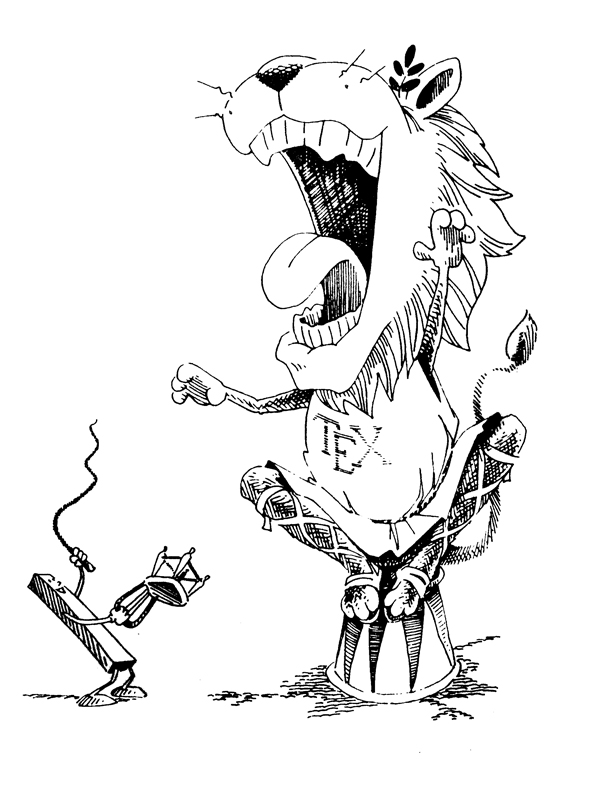
\includegraphics[width=\textwidth]{controlling_TeX_800x600}
	\end{minipage}}

\begin{frame}[fragile]
	\frametitle{Caixas de parágrafo}
	
	\begin{block}{}
		
		\cs{begin}\verb|{minipage}[|%
			\textit{alinhamento}%
		\verb|]{|%
			\textit{largura}%
		\verb|}|
		
		\hspace{1em}\textit{\textbf{caixa}}%
		
		\cs{end}\verb|{minipage}|
	\end{block}
	
	\begin{atividade}<2->{5}
	\setlength{\fboxsep}{0pt}
	
		\smallskip
	
		\noindent\hrulefill
		\usebox{\myminipageA}%
		\hrulefill
		\fbox{\usebox{\myminipageB}}%
		\hrulefill
		
	\end{atividade}
		
\end{frame}
%-------------------------------------------------------------------
\subsection{Linhas}
\begin{frame}[fragile]
	\frametitle{Linhas ou \foreign{rules}}
	
	\begin{block}{}
		\centering
		\cs{rule}\verb|[|%
			\textit{elevação}%
		\verb|]{|%
			\textit{largura}%
		\verb|}{|%
			\textit{altura}%
		\verb|}|
	\end{block}
	
	\begin{columns}
		\column{0.5\textwidth}
	
		\newcolumntype{C}{>{\centering\arraybackslash}X}
		\begin{tabularx}{\textwidth}{Cc}
			\rule[-2.5mm+1ex]{0pt}{5mm}
			\cs{rule}\verb|{5mm}{5mm}| & \rule[-2.5mm+1ex]{5mm}{5mm} \\
			\rule[-2.5mm+1ex]{0pt}{5mm}
			\cs{rule}\verb|{5mm}{1mm}| & \rule[1ex-0.5mm]{5mm}{1mm} \\
			\rule[-2.5mm+1ex]{0pt}{5mm}
			\cs{rule}\verb|{1mm}{5mm}| & \rule[-2.5mm+1ex]{1mm}{5mm}
		\end{tabularx}
	
		\column{0.5\textwidth}
		\flushright
		\uncover<2->{\begin{tikzpicture}[scale=1]
	
	\coordinate (ll) at (0,0);
	\coordinate (ul) at (0,2);
	\coordinate (lr) at (1,0);
	\coordinate (ur) at (1,2);
	\coordinate (dx) at (0.05,0);
	\coordinate (dy) at (0,0.05);
	
	% A caixa-preta (\rule)
	\fill (ll) rectangle (ur);
	
	% A linha-base
	\draw [blue] ($(ll)-(0,1)-10*(dx)$) -- ($(lr)-(0,1)+10*(dx)$);
	
	% A caixa
	\draw [red] ($(0,-1)-(dx)$) rectangle ($(ur)+(dx)+(dy)$);		
	
	% O ponto-de-referência final
	\fill ($(0,-1)$) circle (0.1);
	
	% O ponto-de-referência inicial
	\fill [draw=black,fill=gray] (ll) circle (0.1);
	
	% A flecha da altura
	\draw [<->] ($(lr)+4*(dx)$) -- ($(ur)+4*(dx)$);
	
	% A flecha da largura
	\draw [<->] ($(ul)+4*(dy)$) -- ($(ur)+4*(dy)$);
	
	% A flecha da elevação
	\draw [<->] ($(0,-1)-4*(dx)$) -- ($(ll)-4*(dx)$);
	
	% Rótulo "Altura"
	\node [label=right:Altura] at ($(lr) ! 0.5 ! (ur)$) {};
	
	% Rótulo "Largura"
	\node [label=above:Largura] at ($(ul) ! 0.5 ! (ur)$) {};
	
	% Rótulo "Elevação"
	\node [label=left:Elevação] at ($(0,-1) ! 0.5 ! (ll)$) {};
	
\end{tikzpicture}}
	\end{columns}

	\vspace{-2ex}

	\begin{columns}
		\column{0.6\textwidth}
			\begin{atividade}<3->{6}
				\begin{LaTeXcode}
					texto \rule[+1ex]{1ex}{1ex}
					      \rule[+0ex]{1ex}{1ex}
					      \rule[-1ex]{1ex}{1ex} texto
				\end{LaTeXcode}		
			\end{atividade}
		
		\column{0.4\textwidth}
			\setlength{\fboxsep}{0pt}
		
			\centering
			\Large
			\uncover<3>{
			texto \rule[+1ex]{1ex}{1ex}
			      \rule[+0ex]{1ex}{1ex}
			      \rule[-1ex]{1ex}{1ex} texto}%
			\llap{\uncover<4>{%
			texto {\color{red}
				\framebox[1ex]{\color{gray!50}\rule[+1ex]{1ex}{1ex}}
				\framebox[1ex]{\color{gray!50}\rule[+0ex]{1ex}{1ex}}
				\framebox[1ex]{\color{gray!50}\rule[-1ex]{1ex}{1ex}}} texto}}
	\end{columns}
	
\end{frame}
%-------------------------------------------------------------------
\savebox{\myparboxA}{%
	\parbox{0.32\textwidth}{\tiny\lipsum[4]}}

\subsection{Reutilização de caixas}
\begin{frame}[fragile]
	\frametitle{Reutilizando caixas}
	
	\begin{block}{}
		\cs{newsavebox}\verb|{\|\textit{nome}\verb|}|\\
		\cs{savebox}\verb|{\|\textit{nome}%
		\verb|}[|%
			\textit{largura}%
		\verb|][|%
			\textit{alinhamento}%
		\verb|]{|%
			\textit{\textbf{caixa}}%
		\verb|}|\\
		\dots\\
		\cs{usebox}\verb|{\|\textit{nome}\verb|}|
	\end{block}
	
	\begin{atividade}<2->{7}
		\centering
		Crie e salve uma caixa de parágrafo, e utilize-a\\ três vezes \emph{numa
		mesma linha}. Por exemplo:
	
		\smallskip
	
		\usebox{\myparboxA}\hfill
		\usebox{\myparboxA}\hfill
		\usebox{\myparboxA}
	\end{atividade}
	
\end{frame}
%-------------------------------------------------------------------
\subsection{Medindo caixas}
\begin{frame}[fragile]
	\frametitle{Medindo caixas}
	
	\begin{block}{}
		\cs{settowidth}\verb| {\|%
			\textit{comprimento}%
		\verb|}{|%
			\textit{\textbf{caixa}}%
		\verb|}|\\
		\cs{settoheight}\verb|{\|%
			\textit{comprimento}%
		\verb|}{|%
			\textit{\textbf{caixa}}%
		\verb|}|\\
		\cs{settodepth}\verb| {\|%
			\textit{comprimento}%
		\verb|}{|%
			\textit{\textbf{caixa}}%
		\verb|}|
	\end{block}
	
	\begin{block}<2->{Exercício 3\hspace*{\stretch{1}}\hyperlink{respostas}{\footnotesize\textbf{(resposta)}}}
		Qual é a altura, profundidade e largura da caixa que você criou na atividade anterior?
		
		\medskip
		\footnotesize
		\textbf{obs.:} utilize o comando \cs{the} para imprimir os comprimentos. Por exemplo: \cs{the}\cs{altura} imprime o comprimento \cs{altura} (não use chaves ao redor do argumento).
	\end{block}
	
	\begin{block}<3->{Exercício 4\hspace*{\stretch{1}}\hyperlink{respostas}{\footnotesize\textbf{(resposta)}}}
		Qual é a altura total da caixa do exercício anterior?
		
		\medskip
		\footnotesize
		\textbf{dica:} o comando \cs{addtolength}\verb|{|\textit{comprimento 
		1}\verb|}{|\textit{comprimento 2}\verb|}| adiciona os comprimentos
		1 e 2 e atribui o resultado ao \textit{comprimento 1}.
	\end{block}
	
\end{frame}
%-------------------------------------------------------------------
\subsection{Rotações e redimensionamento}
\begin{frame}[fragile]
	\frametitle{Rotações e redimensionamento de caixas}

	\centering

	Os comandos abaixo requerem o pacote \pkg{graphicx}

	\vfill

	\begin{columns}
		\column{0.6\textwidth}
		\begin{atividade}{8}
			Rotação:\\
			\cs{rotatebox}\verb|{|%
				\textit{ângulo}%
			\verb|}{|%
				\textit{\textbf{caixa}}%
			\verb|}|
			
			\bigskip
		
			Redimensionamento:\\		
			\cs{scalebox}\verb|{|%
				$f_x$%			
			\verb|}[|%
				$f_y$%
			\verb|]{|%
				\textit{\textbf{caixa}}%
			\verb|}|		
			\cs{resizebox}\verb|{|%
				$\ell_x$%
			\verb|}{|%
				$\ell_y$%
			\verb|}{|%
				\textit{\textbf{caixa}}%
			\verb|}|
		\end{atividade}
		
		\column{0.3\textwidth}
		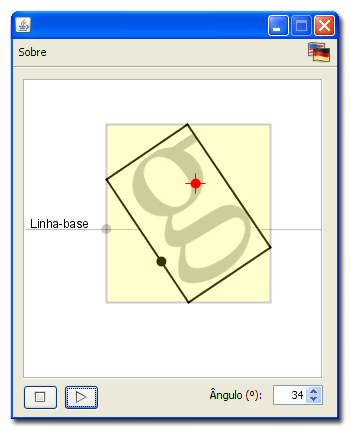
\includegraphics[width=\textwidth]{TeXbox_rotation}
	\end{columns}

	\vfill 

	\textbf{obs.:} comprimentos, contadores e caixas têm escopo global

\end{frame}
%-------------------------------------------------------------------
\ifhandout\else
{
	\logo{
\includegraphics[width=0.25\textwidth]{LogotipoCursoLaTeX_v3_pequeno}}
	\setbeamertemplate{background canvas}{}
	\againframe{titulo} % Reapresenta a página inicial.
}
\fi
%-------------------------------------------------------------------
%-------------------------------------------------------------------
%-------------------------------------------------------------------
\appendix
\section{Respostas}
\begin{frame}[fragile,label=respostas]
	\frametitle{Respostas dos exercícios}

	\footnotesize

	\begin{enumerate}
	\item%
		\begin{LaTeXcode}
		\setlength{\fboxrule}{2pt}
		\setlength{\fboxsep}{0.5mm}
		\fbox{$  \sec^2\theta = 1 + \tan^2\theta  $}
		\end{LaTeXcode}
		
	\item%
		\begin{LaTeXcode}
		\framebox[0.75\textwidth][c]{\(a^2 - b^2 = (a-b)(a+b)\)}
		\end{LaTeXcode}
		
	\item%
		\begin{LaTeXcode}
		\newlength{\altura}
		\settoheight{\altura}{\usebox{\minhacaixa}}
		Altura: \the\altura % <-- Imprime a altura
		
		\newlength{\profundidade}
		\settodepth{\profundidade}{\usebox{\minhacaixa}}
		Profundidade: \the\profundidade
		
		\newlength{\largura}
		\settowidth{\largura}{\usebox{\minhacaixa}}
		Largura: \the\largura
		\end{LaTeXcode}
		
	\item%
		\begin{LaTeXcode}
		\newlength{\alturatotal}
		\setlength{\alturatotal}{\altura}
		\addtolength{\alturatotal}{\profundidade} % altura + profundidade
		Altura total: \the\alturatotal
		\end{LaTeXcode}
	\end{enumerate}

\end{frame}
\end{document}